%%
%% This is file `sample-sigconf.tex',
%% generated with the docstrip utility.
%%
%% The original source files were:
%%
%% samples.dtx  (with options: `sigconf')
%%
%% IMPORTANT NOTICE:
%%
%% For the copyright see the source file.
%%
%% Any modified versions of this file must be renamed
%% with new filenames distinct from sample-sigconf.tex.
%%
%% For distribution of the original source see the terms
%% for copying and modification in the file samples.dtx.
%%
%% This generated file may be distributed as long as the
%% original source files, as listed above, are part of the
%% same distribution. (The sources need not necessarily be
%% in the same archive or directory.)
%%
\PassOptionsToPackage{dvipsnames}{xcolor}
%% The first command in your LaTeX source must be the \documentclass command.
\documentclass[sigconf]{acmart}
\settopmatter{printacmref=false} % Removes citation information below abstract
\renewcommand\footnotetextcopyrightpermission[1]{} % removes footnote with conference information in first column
\pagestyle{plain} % removes running headers

\usepackage{amsmath,amssymb,amsfonts}
\usepackage{graphicx}
\usepackage{textcomp}
%\usepackage[dvipsnames]{xcolor}
\usepackage{minted}
\usepackage{caption}
\usepackage{subcaption}
\usepackage{booktabs}
\usepackage{tikz-timing}
\usepackage{microtype}
\usepackage{float}
\usetikztiminglibrary{arrows}
\usetikztiminglibrary[rising arrows]{clockarrows}
\usetikztiminglibrary{nicetabs}

\usepackage{algorithm}
\usepackage[noend]{algpseudocode}

\graphicspath{{./figs/}}

%%
%% \BibTeX command to typeset BibTeX logo in the docs
\AtBeginDocument{%
  \providecommand\BibTeX{{%
    \normalfont B\kern-0.5em{\scshape i\kern-0.25em b}\kern-0.8em\TeX}}}

%% Rights management information.  This information is sent to you
%% when you complete the rights form.  These commands have SAMPLE
%% values in them; it is your responsibility as an author to replace
%% the commands and values with those provided to you when you
%% complete the rights form.
\acmConference[290 Project]{}{}{}

%%
%% Submission ID.
%% Use this when submitting an article to a sponsored event. You'll
%% receive a unique submission ID from the organizers
%% of the event, and this ID should be used as the parameter to this command.
%%\acmSubmissionID{123-A56-BU3}

%%
%% The majority of ACM publications use numbered citations and
%% references.  The command \citestyle{authoryear} switches to the
%% "author year" style.
%%
%% If you are preparing content for an event
%% sponsored by ACM SIGGRAPH, you must use the "author year" style of
%% citations and references.
%% Uncommenting
%% the next command will enable that style.
%%\citestyle{acmauthoryear}

%%
%% end of the preamble, start of the body of the document source.
\begin{document}

%%
%% The "title" command has an optional parameter,
%% allowing the author to define a "short title" to be used in page headers.
%\title{The Name of the Title is Hope}
\title{Power Modeling and Estimation for Gemmini}

%%
%% The "author" command and its associated commands are used to define
%% the authors and their affiliations.
%% Of note is the shared affiliation of the first two authors, and the
%% "authornote" and "authornotemark" commands
%% used to denote shared contribution to the research.
\author{Vighnesh Iyer}
\email{vighnesh.iyer@berkeley.edu}
\affiliation{%
  \institution{University of California, Berkeley}
}

\author{Billy Chau}
\email{chunheichau@berkeley.edu}
\affiliation{%
  \institution{University of California, Berkeley}
}

%%
%% By default, the full list of authors will be used in the page
%% headers. Often, this list is too long, and will overlap
%% other information printed in the page headers. This command allows
%% the author to define a more concise list
%% of authors' names for this purpose.
%\renewcommand{\shortauthors}{Trovato and Tobin, et al.}

%%
%% The abstract is a short summary of the work to be presented in the
%% article.
\begin{abstract}
  This project seeks to develop an architectural power model for Gemmini based on a macroblock characterization flow.
  The power model will be validated against synthesized implementations of Gemmini running microbenchmarks.
  The model will be used to evaluate the energy breakdown of more complex software and benchmark Gemmini against other ML accelerators.
\end{abstract}

\maketitle

\section{Background and Prior Work}
There are several techniques used in prior work to evaluate power metrics for a digital architecture.
These techniques can be compared and contrasted across the visibility/granularity, fidelity/accuracy, speed, and startup time axes as shown in table \ref{}.

\subsection{Architecture-level Power Modeling}\label{arch_modeling}
This technique typically involves embedding a power model into a functional model of a digital design, or by simulating an abstract architecture description against an abstract software model/activity counts.

Examples for the former technique include the power models used for evaluating the Eyeriss v2\cite{eyerissv2} and SCNN\cite{scnn} architectures which were implemented by counting SRAM reads/writes, MACs, NoC metrics, and DRAM accesses within the functional model, and assigning an energy/op number to each type of op.
Some refinements to the power model were made by accounting for the impact of sparsity on MAC power (clock gating), the power usage of crossbars, FIFOs, and other auxiliary control circuits, and using a cycle-accurate performance model to capture non-idealities such as DRAM and NoC latency and multi-cycle arithmetic.

An example of the latter technique is Accelergy\cite{accelergy}, which is a framework for estimating power from an architectural description of a tiled PE accelerator, a description of the digital components for that architecture (SRAMs, registers, MAC/multiply/adder blocks, FIFOs, crossbars, NoC routers, etc.), and plugins for defining the power models of each architectural component depending on what actions are performed on them.
Accelergy is fed by a performance model which produces activity counts accounting for memory, compute, and communication latencies.
Another example of an architectural power model using an abstract architecture description is the gem5 power simulator\cite{gem5power}.

Architecture-level modeling is generally fast, but can suffer from low accuracy if $\mu$Arch details aren't properly considered or if the per-component power models aren't properly characterized. However, for ML accelerators, due to the regularity of computation and memory movement, architecture power models can be quite accurate. In the context of Gemmini, such a model may have accuracy loss due to non-consideration of CPU power, and performance variation from SoC integration (the effect of the shared L2 cache with the CPU, the impact of coherence from L1 and fencing, threading, and interrupts).

\subsubsection{RTL Macromodeling}
To generate the component-level power models for use in architectural simulation, RTL macromodeling is used.
The idea is to create a function ($f(\text{input statistic}) = \text{predicted energy}$) that can map some statistics about the input to a macroblock to the energy consumed by the block to process the input.
Concretely, this would be a map from input data sparsity to dynamic energy for an arithmetic block, a fixed cost model for SRAMs (accounting for re-reading the same address), and an activity-based model for registers.
The model also accounts for leakage energy that is expended every cycle.

\subsection{Post-Synthesis Vectored Power Simulation}\label{syn_modeling}
This flow is supported by Cadence Joules and involves taking an RTL design through synthesis and measuring power from a VCD generated by gate-level simulation.
This technique is relatively fast compared to the signoff power flow, but requires a full RTL design and a synthesized netlist.
It is relatively accurate, but can only estimate the layout parasitics from a partial sketch of the floorplan.

\subsection{Post-PnR Vectored Power Simulation}
This flow is supported by Cadence Voltus and requires the RTL to be fully implemented to function; furthermore a post-pnr gate-level sim is required which runs very slowly (~100 Hz).
However, the signoff power estimated by this flow is as accurate as one can get and you can get precise current waveforms for each net.

\subsection{Chip measurement}
Taking an architecture to tapeout will get the most accurate power numbers, will be able to run software in realtime, but you will only be able to evaluate a few corners, supplies, and frequencies with only one design point.
A chip also has poor visibility and getting module-level power numbers is not possible.

\section{Approach and Results}

\subsection{Proposed Flow}
We propose a flow that combines the techniques from Sections \ref{arch_modeling} and \ref{syn_modeling} in Figure \ref{fig:overall_flow}.
We set out to perform macroblock power characterization on the most power hungry units of Gemmini (MAC, registers, and SRAM), apply those numbers to an embedded power model in Gemmini's functional simulator, validate the power estimates from the arch power simulator against post-synthesis power estimation, and finally attempt to model Gemmini in Accelergy as an additional point of validation.

\begin{figure}
  \begin{center}
    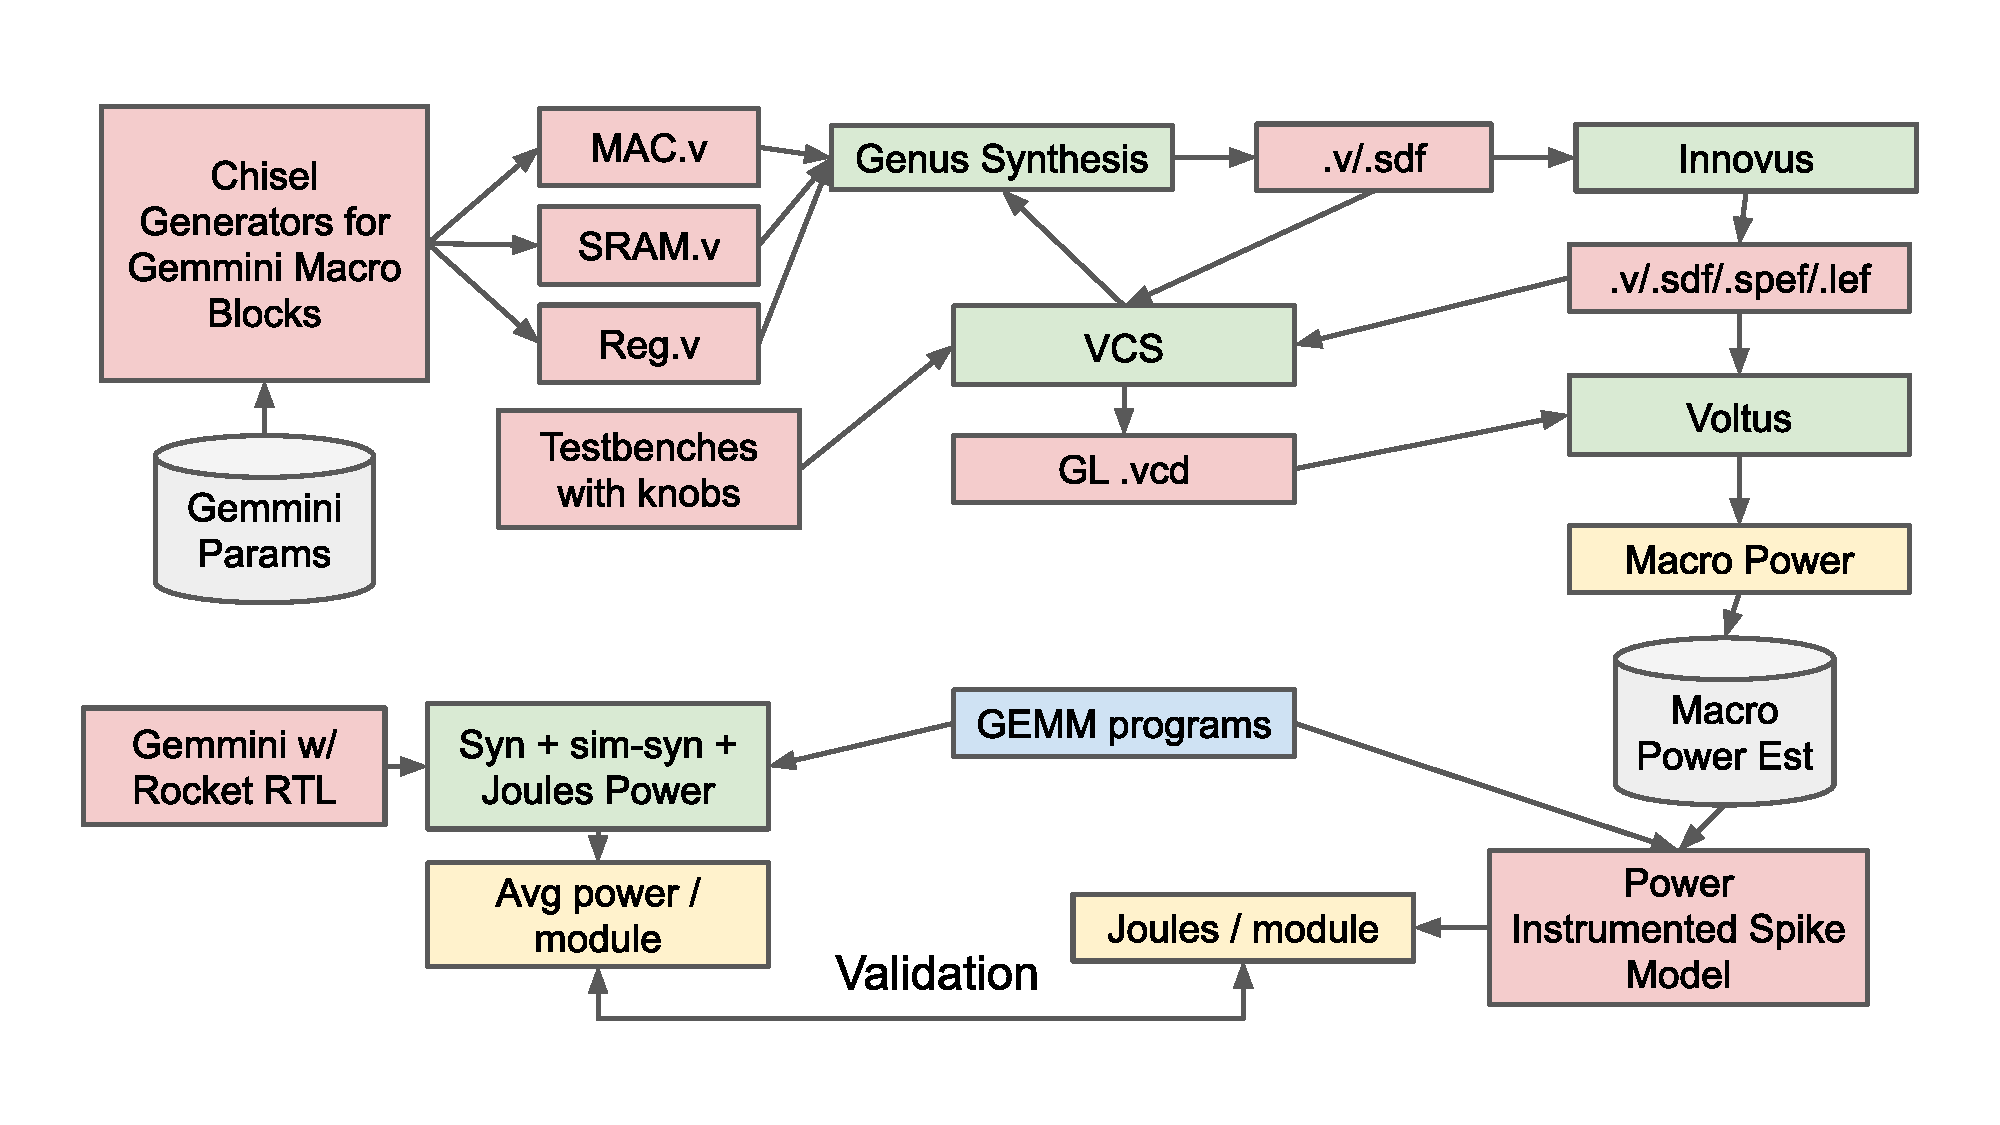
\includegraphics[width=\linewidth]{overall_flow.pdf}
  \end{center}
  \caption{Description of the proposed flow consisting of macroblock modeling, activity instrumentation of a functional model, and validation with Joules}
\end{figure}

\subsection{Macroblock Power Modeling}
We propose macroblock modeling of a few power-critical blocks of Gemmini such as the MAC and SRAM units that make up the accumulator and scratchpad.
We can extract the register write energy from the MAC macromodeling as described below.

The macroblock modeling flow starts with Chisel generators that mimic the power-critical modules of Gemmini and are parameterized similar to Gemmini.
These blocks are pushed through the standard VLSI flow to produce post-pnr views.
A post-pnr timing annotated gate-level simulation is run with a testbench that can vary the module's input stimulus.
The VCD produced by VCS is fed to Voltus along with the extracted post-pnr design to extract average power.

\subsubsection{MAC and Registers}
We modeled an integer MAC within a PE of Gemmini using its \texttt{Arithmetic} typeclass and accounting for the differences between the output and weight stationary configurations:

\begin{minted}[breaklines,fontsize=\small]{scala}
class MACConfig[T <: Data:Arithmetic](val aType: T, val bType: T, val cType: T)
// In OS mode: a and b are 8 bits and c is 32 bits of the internal accumulator
// In WS mode: a and b are also 8 bits, but c is 19 bits of the PE from above
case class OSMACConfig() extends MACConfig(SInt(8.W), SInt(8.W), SInt(32.W))
case class WSMACConfig() extends MACConfig(SInt(8.W), SInt(8.W), SInt(19.W))
\end{minted}

The \texttt{MAC} module consisted of input registers for the \texttt{a}, \texttt{b}, and \texttt{c} operands, the actual MAC ($c_{out} = a*b + c$), and an output register for the result $c_{out}$.
The inputs and outputs were registers to allow us to constrain the timing of the MAC and to create an environment similar to Gemmini's PE.

The \texttt{MAC} module was driven by a testbench that could control the input density of \texttt{a} and \texttt{b} to model input activation and weight sparsity for the weight stationary dataflow.
The testbench models the weight stationary dataflow by keeping \texttt{b} stationary for 16 cycles (the default Gemmini \texttt{DIM}) at a time and allowing \texttt{a} to change every cycle.
The testbench was written in Verilog instead of from within Scala (using \texttt{chisel-iotesters}/\texttt{chiseltest}) to enable easy integration with gate-level simulation.
Future work involves porting the testbench to Scala after gate-level simulation support is available to enable easy propagation of generator parameters to the testbench.

We produce results from Voltus for a 100\% dense input sequence and a weight-stationary MAC configuration shown in Figure \ref{fig:mac_energy}.

\begin{figure}
\begin{tabular}{l l l l l}
  \textbf{Group} & \textbf{Internal} & \textbf{Switching} & \textbf{Leakage} & \textbf{Total} \\
  \toprule
  Sequential & 0.08327 & 0.01127 & 0.01612 & 0.1107 \\ \midrule
  Combinational & 0.06096 & 0.04821 & 0.01616 & 0.1253 \\
  \bottomrule
\end{tabular}
\caption{Power numbers for a registered 8/8/19 bit SInt MAC, all numbers in mW}
\label{fig:mac_energy}
\end{figure}

The testbench runs for 1600 cycles and the MAC was timed at 1 GHz.
The total energy per MAC is then around \textbf{125 fJ} and the energy per register write per bit is \textbf{2 fJ}.
The leakage energy per MAC per cycle is \textbf{16 fJ}.
During the entire waveform the total power of the MAC + registers ranged between 0.14 mW and 0.34 mW in 2ns intervals.

We also examine the impact of changing the input densities of \texttt{a} and \texttt{b} in Figure \ref{fig:density_mac}.
Different input densities had a minimal impact on sequential power, but reduced dynamic combinational power linearly with the density reduction.
Unsurprisingly, reducing density in the weight matrix had a larger impact than density in the input activations due to the weight stationary dataflow that's being assumed.

\begin{figure}
\begin{tabular}{l l l}
  \textbf{Input Density} & \textbf{fJ/MAC (a)} & \textbf{fJ/MAC (b)} \\
  \toprule
  1 & 125 & 125 \\ \midrule
  0.875 & 121 & 97 \\ \midrule
  0.5 & 107 & 81 \\ \midrule
  0.125 & 84 & 67 \\ \midrule
  0 & 70 & 60 \\
  \bottomrule
\end{tabular}
\caption{Impact of different densities of \texttt{a} and \texttt{b} on MAC energy in a WS enviroment}
\label{fig:density_mac}
\end{figure}




% keep raw data here, but commented out
\iffalse
changing density of a (affects every cycle)

7/8 density = 121 fJ
Sequential                     0.08286      0.01106       0.01613      0.1101       47.59
Macro                                0            0             0           0           0
IO                                   0            0             0           0           0
Combinational                  0.05868      0.04644        0.0161      0.1212       52.41

4/8 density = 107 fJ
Sequential                     0.08256       0.0101       0.01611      0.1088       50.31
Macro                                0            0             0           0           0
IO                                   0            0             0           0           0
Combinational                  0.05111      0.04038       0.01594      0.1074       49.69

1/8 density = 84 fJ
Sequential                     0.08236     0.008656       0.01611      0.1071       55.91
Macro                                0            0             0           0           0
IO                                   0            0             0           0           0
Combinational                  0.03821      0.03021       0.01606     0.08449       44.09

0/8 density = 70 fJ
Sequential                     0.08196     0.007843       0.01609      0.1059       60.14
Macro                                0            0             0           0           0
IO                                   0            0             0           0           0
Combinational                  0.03016      0.02391       0.01611     0.07018       39.86

changing density of b (affects 16 cycle blocks)
7/8 density = 97 fJ
Sequential                     0.08199        0.011       0.01612      0.1091        52.9
Macro                                0            0             0           0           0
IO                                   0            0             0           0           0
Combinational                  0.04556      0.03558       0.01599     0.09713        47.1

4/8 density = 81 fJ
Sequential                     0.08156      0.01115       0.01612      0.1088       57.24
Macro                                0            0             0           0           0
IO                                   0            0             0           0           0
Combinational                  0.03707      0.02838       0.01584     0.08128       42.76

1/8 density = 67 fJ
Sequential                     0.08096      0.01101       0.01611      0.1081       61.67
Macro                                0            0             0           0           0
IO                                   0            0             0           0           0
Combinational                  0.02963      0.02203       0.01552     0.06719       38.33

0/8 density = 60 fJ
Sequential                     0.08049       0.0109        0.0161      0.1075       64.08
Macro                                0            0             0           0           0
IO                                   0            0             0           0           0
Combinational                  0.02586      0.01894       0.01545     0.06024       35.92
\fi

\subsubsection{SRAM Macromodeling}


\subsection{Spike Power Model}

\subsection{Gemmini Post-Syn Joules Evaluation}

\subsection{Modeling Gemmini in Acceleregy}
\subsubsection{Gemmini Accelergy Model}
We modeled Gemmini's architecture as a combination of two scratchpads (weight and input), one accumulator scratchpad, and 16x16 PE elements; each with 8 bits integer MAC unit and register.

\begin{minted}[breaklines,fontsize=\small,frame=single]{yaml} 
architecture:
  version: 0.3
  subtree:
    - name: eyeriss_like
      attributes:
        technology: 65nm
      local:
        - name: weights_sp
          class: SRAM
          attributes:
            width: 128
            depth: 4096
            n_banks: 2
            n_rdwr_ports: 1
        - name: ifmap_sp
          class: SRAM
          attributes:
            width: 128
            depth: 4096
            n_banks: 2
            n_rdwr_ports: 1
        - name: accum_sp
          class: SRAM
          attributes:
            width: 512
            n_banks: 1
            bank_depth: 1024
            depth: bank_depth * n_banks
            n_rdwr_ports: 1
      subtree:
      - name: PE[0..255]
        local:
          - name: weight_or_output
            class: reg
            attributes:
              datawidth: 8
          - name: mac
            class: intmac
            attributes:
              datawidth: 8
          - name: pipeline_reg
            class: reg
            attributes:
              datawidth: 8
\end{minted}

\subsubsection{Future Work}
The current model lacks of fidelity as it does not account for the behavior of the L2 cache, double buffering, wire, etc., so it will be a good idea to refine the existing model in the future.

\section{Conclusion}

\appendix
\section{Links}
% chipyard branch
% esp-isa-sim fork
% this repo
% models used for Accelergy

\section{Original Proposal}

\subsection{Modifications / Rationale}


The architecture and VLSI literature has produced a litany of dedicated ML accelerators over the last 3 years.
These accelerators exploited unique dataflows, weight/activation sparsity, integer arithmetic, novel circuit techniques, or other techniques to achieve a perf/watt advantage over a baseline design.

However, architecture papers typically measure the energy consumption of the proposed accelerator against a baseline using a (Python/C++) model of their accelerator, and thus produce unreliable energy numbers.
Some papers use HLS to generate RTL implementations of different architectures.
The RTL is synthesized and RTL simulation is used to produce activity traces for energy estimation.
Unfortunately, RTL simulation is slow, and thus only small DNNs can be evaluated.

On the other hand, chip/VLSI papers measure the energy consumption of a taped out chip, but do not have a baseline accelerator implementation taped-out to compare against.
Furthermore, once a chip is taped out, the power consumption cannot be measured for individual parts of the accelerator (at module-granularity) and cycle-by-cycle energy numbers cannot be extracted.

\section{Prior Work}
STROBER\cite{strober} is a fast and cycle-accurate sample-based energy estimation framework that automatically transforms RTL into a deterministic FPGA simulator.
The work instruments the RTL design with a shadow scan chain that enables $\mu$Arch state extraction by the host.
To estimate energy, STROBER exploits the central limit theorem by taking state snapshots of the RTL at intervals using reservoir sampling and replaying those snapshots on a gate-level power simulator.
%It has achieved less than
%5 percents error with 99.9 percents confidence against commercial CAD tools with more
%than two orders of magnitude speedup over existing microarchitectural simulators and
%four orders of magnitude speedup over commercial Verilog simulators.

%\textbf{Highlights}

%State Snapshotting using Scan Chain - As detailed information of simulation is required
%for an accurate power model, a basic scan chain is embedded into the design to capture
%a replayable RTL snapshot with both register and SRAM values. Using the hardware
%construction language Chisel, all custom transforms and FAME1 transform can be easily
%mapped and wrapped around the RTL design.

%Sample-based Energy Simulation - Based on the central limit theorem of statistics,
%a representative estimator of the power model can be generated given random sampling
%and enough snapshot samples. However, knowing the length of the program's execution
%is impossible, so the reservoir sampling technique is used to address this problem.

%Fine-grained level Simulation and Checking - Independent replayable snapshots are replayed in parallel in
%commercial gate-level simulators such as VCS for accurate power analysis. To ensure the correctness of the execution, the output values
%of the design are compared with the output traces.

Simmani\cite{simmani} is a framework that trains a power model that takes toggle activity for a small subset of signals in the RTL design (found via clustering on signal toggle densities from training VCDs), instruments the RTL design with activity counters for these signals, and enables runtime power estimation.
This work demonstrated good power accuracy on running SqueezeNet on Rocket with a Hwacha vector accelerator.
%Simmani\autocite{simmani} is an FPGA-accelerated framework which automatically selects signals most correlated with power dissipation and trains power models in terms of the selected signals for any RTL design. It has achieved accurate power models with acceptable errors on real world machine learning application such as SqueezeNet running with Rocket Core and Hwacha Vector Accelerator.

%\textbf{Highlights}

%Activity Counter Insertion and FPGA accelerated simulation - Utilizing the Strober framework, any RTL designs are automatically transformed for FPGA-accelerated RTL simulation. The framework is also used to obtain runtime power traces from FPGAs by inserting activity counters.

%Toggle Density Matrix with Principal Components Projection - In order to train an accurate power model, toggle pattern matrix is used to represent signals and their toggle frequencies. The intuition behind is that signals showing similar toggle patterns have similar effect on dynamic power dissipation and can be factored to share the same coefficient in the power model, thus minimizing modeling error. However, it suffers from the curse of dimensionality like other machine learning algorithms; therefore, SVD-based dimensionality reduction algorithm is used to extract the top k dimensions.

%Automatic Signal Selection - Given N, the number of signals selected from Bayesian Information Criterion, k-means++ algorithm is run to cluster the signals into groups i.e. signals with similar toggle pattern are grouped together. Then, the signals that are the closest to the center of each cluster are selected, which will be the regression variables in power model training.

%Power Model Regression - Using Elastic Net for variable regularization and selection with k-fold cross-validated hyperparameters, a regression model is trained using the toggle density matrix and the groud truth power traces obtained from commercial CAD tools calculated from RTL VCD dumps.

DESSERT\cite{dessert} is a framework for FPGA-accelerated RTL debugging that enables synthesized assertions and full $\mu$Arch state dumping.
This work demonstrates the flexibility of a instrumented scan chain to dump arbitrary state that we could use to ``instrument" the RTL design in software after a bitstream has already been created.
%DESSERT\autocite{dessert} is an FPGA-accelerated framework for effective simulation-based RTL verification and debugging. It has achieved almost no performance overhead with hardware-based assertion checking and insignificant performance overhead for software-based exhaustive checking in comparison to commercial CAD tools.

%\textbf{Highlights}

%Error Capturing using Scan Chain - Following the technique in the Strober framework, scan chain based snapshotting is used for error capturing in DESSERT. There are two constructs supporting assertion and logs in FIRRTL: stop and printf, and they are mapped automatically from the source code by DESSERT. In order to detect and replay errors efficiently, two identical and deterministic simulators are run in parallel. The leading master instance is to detect the target RTL bugs while the lagging instance is to checkpoint the target RTL state.

%Software-based Golden Model Checking - When the logs are generated from FPGA, they are sent to the
%buffers in the software simulation driver through DMA. They are then compared with a software-based golden model such as Spike for exhaustive error checking.

\section{Proposal}
We propose a framework that enables:
\begin{itemize}
  \item RTL-fidelity simulation of ML accelerators over full DNN inference passes

    We plan to re-use the Firesim FIRRTL passes that automatically transform arbitrary RTL to a deterministic, cycle-accurate model that executes on an FPGA.

  \item Gate-level fidelity energy modeling (with module-level granularity)

    We plan to modify and add passes to Golden Gate that add a stitched scan chain and SRAM hijack ports that allows the host to inject and pull all $\mu$Arch state to and from the DUT.
    This technique is distinct from DESSERT and STROBER since those works use a shadow scan chain that cannot inject state into the DUT, and may be more resource intensive.

    This allows us to advance simulation time, pause at random intervals, and dump the DUT state to the host, similar to STROBER.
    The randomly sampled RTL-level activity traces can be formally mapped into gate-level traces and fed into Voltus with a gate-level synthesized netlist for cycle-by-cycle energy estimates.

  \item Performance instrumentation and bottleneck analysis (PE utilization, memory traffic analysis)

    We plan to use the auto-instrumentation (AutoCounter) feature in FirePerf\cite{fireperf} to dump design-specific performance counters to evaluate bottlenecks in DNN inference.
    We also plan to instrument the off-chip memory interface to record the DRAM address and transfer size patterns.

  \item Energy estimation of DRAM accesses

    The memory access trace can be replayed in DRAMSim2\cite{dramsim2} to extract average power numbers across time.
    DRAM access energy is sometimes neglected in RTL-level power analyses and but was done in the STROBER flow.

  \item Exploration of the impact different dataflows and tiling patterns on energy and performance

    Finally, once the framework described has been implemented, it can be used to guide software optimizations.
\end{itemize}

We plan to use this framework to evaluate Gemmini\cite{gemmini} and BOOM, and if time permits, NVDLA on Firesim\cite{nvdlafiresim}.

\section{Project Infrastructure}
For the initial phase of the project, we don't require any special infrastructure apart from our laptops and the BWRC servers for Genus/Jasper/Voltus (we hope VPN works).
Once software simulation is successful, we will use some AWS F1 instances.

\section{Project Timeline}

\begin{enumerate}
  \item \textbf{Checkpoint 1 (4/10)}: RTL simulation of a simple circuit (Risc/GCD) after default Firesim transformation, ASAP7 Genus synthesis of the circuit and SRAM macros, formal mapping of RTL VCD to gate-level VCD, scan-chain stitching and SRAM hijack FIRRTL pass working in RTL simulation
  \item \textbf{Checkpoint 2 (4/24)}: Sample circuit simulating on F1 FPGA, $\mu$Arch state dumping, initial energy estimation evaluation
  \item \textbf{Final Report (5/8)}: Rocket with Gemmini simulating on F1 FPGA, DRAM interface and Gemmini-specific performance instrumentation, Gemmini energy estimation for pre-written ResNet50 and Mobilenet implementations, DRAMSim2 energy estimation
\end{enumerate}

The timeline is aggressive and there may be points where we find ourselves stuck.
It is likely that the custom FIRRTL passes introduce difficult to find bugs and may delay this timeline.
It is not clear how to perform formal mapping of RTL VCDs to gate VCDs, but there's probably a Cadence RAK for it.



%%
%% The acknowledgments section is defined using the "acks" environment
%% (and NOT an unnumbered section). This ensures the proper
%% identification of the section in the article metadata, and the
%% consistent spelling of the heading.
%\begin{acks}
%\end{acks}

%%
%% The next two lines define the bibliography style to be used, and
%% the bibliography file.
\bibliographystyle{ACM-Reference-Format}
\bibliography{references}

\end{document}
\endinput
%%
%% End of file `sample-sigconf.tex'.
